\documentclass[11pt,a4paper]{report}
\usepackage[utf8]{inputenc}
\usepackage{amsmath}
\usepackage{amsfonts}
\usepackage{amssymb}
\usepackage{graphicx}
\usepackage{pgfplots}
\usepackage{minted}
\usepackage{mathtools}
\usepackage{pdfpages}
\definecolor{bg}{rgb}{0.95,0.95,0.95}

\title{Relatório Final  \\
	Projeto em Eletrônica I - EEL7801 \\ \vfill
	\normalsize{Universidade Federal de Santa Catarina - UFSC \\
		Professora: Daniela Ota Hisayasu Suzuki}
	\author{
		{Luiz Augusto Frazatto Fernandes: \it{17202752}} \\
		{Leonardo José Held: \it{17203984}}
}
}
\date{6 de Julho de 2019}
\begin{document}
	\maketitle
	\setcounter{chapter}{0}

	
	\chapter{Validação de Algorítmo FSK}
		A implementação algorítmica teve, como principais desafios, a tradução de códigos de alto nível de modulação e demodulação em códigos de baixo nível, bem como a adequação dos códigos aos MCUs escolhidos. A demodulação, no entanto, não fora completamente finalizada por conta de dois fatores:
		\begin{itemize}
			\item[1.] Uma das placas tornou-se irresponsiva e não mais conseguimos programá-la.
			\item[2.] Há a necessidade de grande capacidade de memória RAM para se processar o vetor a ser demodulado. Logo, fizemos o uso de um Raspberry Pi 3.
		\end{itemize}
	O Raspberry Pi executa o código de captura de demodulação do sinal. O STM32 executa a modulação do sinal obtido. O esquemático pode ser encontrado depois da seção de códigos.
		
	\section{Modulação em baixo nível (C/C++)}
		A modulação é realizada através de duas Look Up Tables (LUT) contendo valores de duas funções seno (cada um com uma frequência diferente). Resumidamente: a informação (convertida em binário) é transformada num sinal modulado por FSK.
	\subsection{lut.h}
		\begin{minted}[frame=lines,
		framesep=2mm,
		baselinestretch=1.2,
		bgcolor=bg,
		fontsize=\footnotesize,
		breaklines
		]{c}
#ifndef LUT_H
#define LUT_H
		
#include <stdlib.h>
#include <stdio.h>
		
#define DATA_SIZE 10
		
#define VECTOR_SIZE 6400
		
static const int lut_2T[] = {
0x8,0x9,0xa,0xa,0xb,0xc,0xc,0xd,
0xe,0xe,0xf,0xf,0xf,0x10,0x10,0x10,
0x10,0x10,0x10,0x10,0xf,0xf,0xf,0xe,
0xe,0xd,0xc,0xc,0xb,0xa,0xa,0x9,
0x8,0x7,0x6,0x6,0x5,0x4,0x4,0x3,
0x2,0x2,0x1,0x1,0x1,0x0,0x0,0x0,
0x0,0x0,0x0,0x0,0x1,0x1,0x1,0x2,
0x2,0x3,0x4,0x4,0x5,0x6,0x6,0x7};
		
static const int lut_T[] = {
0x8,0xa,0xb,0xc,0xe,0xf,0xf,0x10,
0x10,0x10,0xf,0xf,0xe,0xc,0xb,0xa,
0x8,0x6,0x5,0x4,0x2,0x1,0x1,0x0,
0x0,0x0,0x1,0x1,0x2,0x4,0x5,0x6};
		
void lut_association(int input_binary_signal[], int **output_analog_signal);
		
#endif
		\end{minted}
		
	\subsection{lut.c}
		\begin{minted}[frame=lines,
		framesep=2mm,
		baselinestretch=1.2,
		bgcolor=bg,
		fontsize=\footnotesize,
		breaklines
		]{c}
#include "lut.h"
		
void lut_association(int input_binary_signal[], int **output_analog_signal)
{
	free(*output_analog_signal);
	*output_analog_signal = malloc(VECTOR_SIZE * sizeof(int));
	if (*output_analog_signal == NULL)	return;
	for (int i = 0; i < DATA_SIZE; i++)	{
		int multiple1 = i * DATA_SIZE * 64;
		if (input_binary_signal[i] == 1)	{
			for (int j = 0; j < DATA_SIZE; j++)	{
				int multiple2 = j * 64;
				for (int k = 0; k < 64; k++)	{
							
					(*output_analog_signal) [multiple1 + multiple2 + k] = lut_T[k % 32];
				}
			}
		}	else	{
			for (int j = 0; j < DATA_SIZE; j++)	{
				int multiple2 = j * 64;
				for (int k = 0; k < 64; k++)	{
					(*output_analog_signal) [multiple1 + multiple2 + k] = lut_2T[k];
				}
			}
		}
	}
}
		\end{minted}
		
	\subsection{mod\_main.c}
		\begin{minted}[frame=lines,
		framesep=2mm,
		baselinestretch=1.2,
		bgcolor=bg,
		fontsize=\footnotesize,
		breaklines
		]{c}
#include "lut.h"
	
int main(void)
{
	int transmitted_data[DATA_SIZE] = {1, 0, 1, 0, 1, 1, 1, 0, 0, 1};
	int *modulated_signal;
		
	modulated_signal = NULL;
	lut_association(transmitted_data, &modulated_signal);
	free(modulated_signal);
		
	return 0;
}
		
		\end{minted}
		
	\section{Aquisição dos dados}
		\begin{minted}[frame=lines,
		framesep=2mm,
		baselinestretch=1.2,
		bgcolor=bg,
		fontsize=\footnotesize,
		breaklines
		]{python}
import time
import board
import busio
import adafruit_ads1x15.ads1115 as ADS
from adafruit_ads1x15.ads1115 import Mode
from adafruit_ads1x15.analog_in import AnalogIn
		
RATE = 860
SAMPLES = 10000
		
# BUS I2C de alta frequencia
i2c = busio.I2C(board.SCL, board.SDA, frequency=1000000)
ads = ADS.ADS1115(i2c)
		
#Pino A0
channel0 = AnalogIn(ads, ADS.P0)
		
ads.mode = Mode.CONTINUOUS
ads.data_rate = RATE
ads.gain = 2/3
		
		
adc_values = [None]*SAMPLES
		
start = time.monotonic()
		
# Lê
for i in range(SAMPLES):
adc_values[i] = channel0.value
#adc_values[i] = channel0.voltage
end = time.monotonic()
total_time = end - start
		
with open('values.txt', 'w') as f:
for item in adc_values:
f.write("%s " % item)
		
print("Tempo de captura: {}s".format(total_time))
		\end{minted}


	\section{Demodulação em baixo nível (C/C++)}
	\paragraph{}
		A demodulação consiste em, a partir dos dados obtidos pelo sensor, interpretar o sinal recebido e identificar a frequência com que esse "cruza" a faixa de DC OFFSET. Calcula-se o valor médio da tensão gerada pelo sinal e, a partir desse, consegue-se identificar diferentes frequências.
		
		O executável do programa, provido de um arquivo texto contendo um sinal modulado, é tal:\\
		
		\texttt{./demod\_main.out\\                                       
			Original vector: [ 1 0 1 0 1 1 1 0 0 1 ]
\\
			Demodulated vector: [ 1 0 1 0 1 1 1 0 0 1 ]
}
		
	
	\subsection{functions.h}
		\begin{minted}[frame=lines,
		framesep=2mm,
		baselinestretch=1.2,
		bgcolor=bg,
		fontsize=\footnotesize,
		breaklines
		]{c}
#include <stdio.h>
#include <stdlib.h>
		
#define BITS 10
#define PERIOD_SAMPLE 2560
#define LENGTH (BITS*PERIOD_SAMPLE)
		
void get_wave(int array[], int size);
		
void analyze_zeros(int wave[], int **zeros, const int nro_bits, const int sampling_period_length, double reference);
		
double get_mean(int vector[], int vector_size);
		
void get_normalized(double normalized_vector[], int vector[], double mean);
		
void print_vector(double vector[]);
		\end{minted}
		
	
	\subsection{functions.c}
		\begin{minted}[frame=lines,
		framesep=2mm,
		baselinestretch=1.2,
		bgcolor=bg,
		fontsize=\footnotesize,
		breaklines
		]{c}
#include "functions.h"
		
void get_wave(int array[], int size)
{
FILE *myfile;
myfile=fopen("new_mod_result.txt", "r");
		
for(int i = 0; i < LENGTH; i++)   {
	fscanf(myfile,"%d", &array[i]);
}
		
fclose(myfile);
		
}
		
void analyze_zeros(int wave[], int **zeros, const int nro_bits, const int sampling_period_length, double reference)
{
	free(*zeros);
	*zeros = malloc(sizeof(int) * nro_bits);
	if (*zeros == NULL) return;
	int zero_sampling[nro_bits];
	int positive = 0;
	int negative = 0;
	int dif_signal = 0;
			
	for (int i = 0; i < nro_bits; i++)  {
		int vector_position = PERIOD_SAMPLE * i;
		zero_sampling[i] = 0;
		for (int j = 0; j < sampling_period_length; j++) {
			if (dif_signal > nro_bits)  {
				if (wave[vector_position + j] > reference)   {
					positive = 1;
				}
				if (wave[vector_position + j] < reference)   {
					negative = 1;
				}
				if (positive && negative)   {
					zero_sampling[i] += 1;
					positive = 0;
					negative = 0;
					dif_signal = 0;
				}
			}
			dif_signal++;
		}
	}
	for (int i = 0; i < BITS; i++){
		(*zeros)[i] = zero_sampling[i];
	}
}
double get_mean(int vector[], int vector_size)
{
	double sum = 0;
	for (int i = 0; i < vector_size; i++)   {
		sum += vector[i];
	}
			
	return sum/vector_size;
}
		
void get_normalized(double normalized_vector[], int vector[], double mean)
{
	for (int i = 0; i < BITS; i++)   {
		normalized_vector[i] = (double)vector[i] / mean;
	}
}
		
void print_vector(double vector[])
{
	printf("Demodulated vector: [ ");
	for (int i = 0; i < BITS; i++)    {
		if (vector[i] > 1)    {
			printf("1 ");
		}   else    printf("0 "); 
	}
	printf("]\n");
}
		\end{minted}
		
		
	\subsection{demod\_main.c}
		\begin{minted}[frame=lines,
		framesep=2mm,
		baselinestretch=1.2,
		bgcolor=bg,
		fontsize=\footnotesize,
		breaklines
		]{c}
#include "functions.h"
		
int main(void)
{
	printf("Original vector (obtained from modulation in C): \
	[ 1 0 1 0 1 1 1 0 0 1 ]\n");
			
	int array[LENGTH];
	int *zeros;
	double normalized_vector[BITS];
	int demodulated_wave[BITS];
			
	get_wave(array, LENGTH);
			
	zeros = NULL;
	analyze_zeros(array, &zeros, BITS, PERIOD_SAMPLE, get_mean(array, LENGTH));
			
	double mean = get_mean(zeros, BITS);
	get_normalized(normalized_vector, zeros, mean);
	print_vector(normalized_vector);
			
	free(zeros);
			
	return 0;
}
		\end{minted}
		
	

	
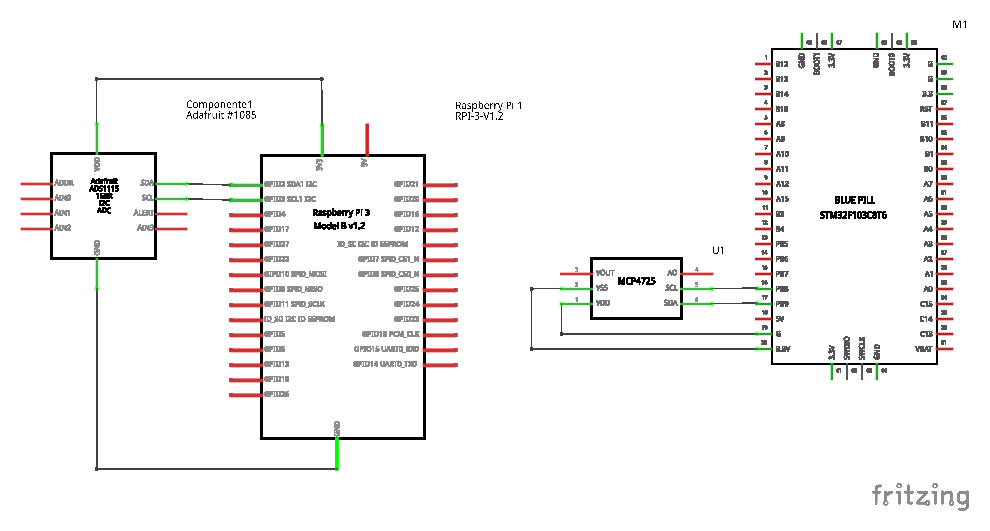
\includepdf{pi_e_bp}
		
		
\chapter{Validação Física}
\section{Modem com transdutores ultrassom}

Aqui dois transdutores de baixa frequência (40Hz) foram utilizados. Um funciona como emissor e outro como receptor microfone. O receptor passa por um amplificador de aúdio (que funciona apenas como amplificador simples), um filtro e um comparador, que checa se o sinal é ativo ou não. O emissor simplesmente usa 5V, e um pino digital do MCU em modo {\it PWM} para gerar a frequência utilizada.

O código do emissor usa uma frequência base para ligar ou desligar a saída com base nos bits dos \texttt(char) programados no texto. Dependendo do tempo de resposta entre a recepção de um sinal, uma interrupção é ativada e um bit é colocado em $1$ ou $0$ de acordo, muito parecido com o comportamento de um sonar. O receptor apenas checa a entrada de um pino digital, que é coloca em alto ou baixo dependendo da saída do comparador.


A vantagem dessa configuração é que ela só depende do tempo entre dois caracteres para saber qual será o próximo, configurando uma comunicação assíncrona.

\begin{center}
	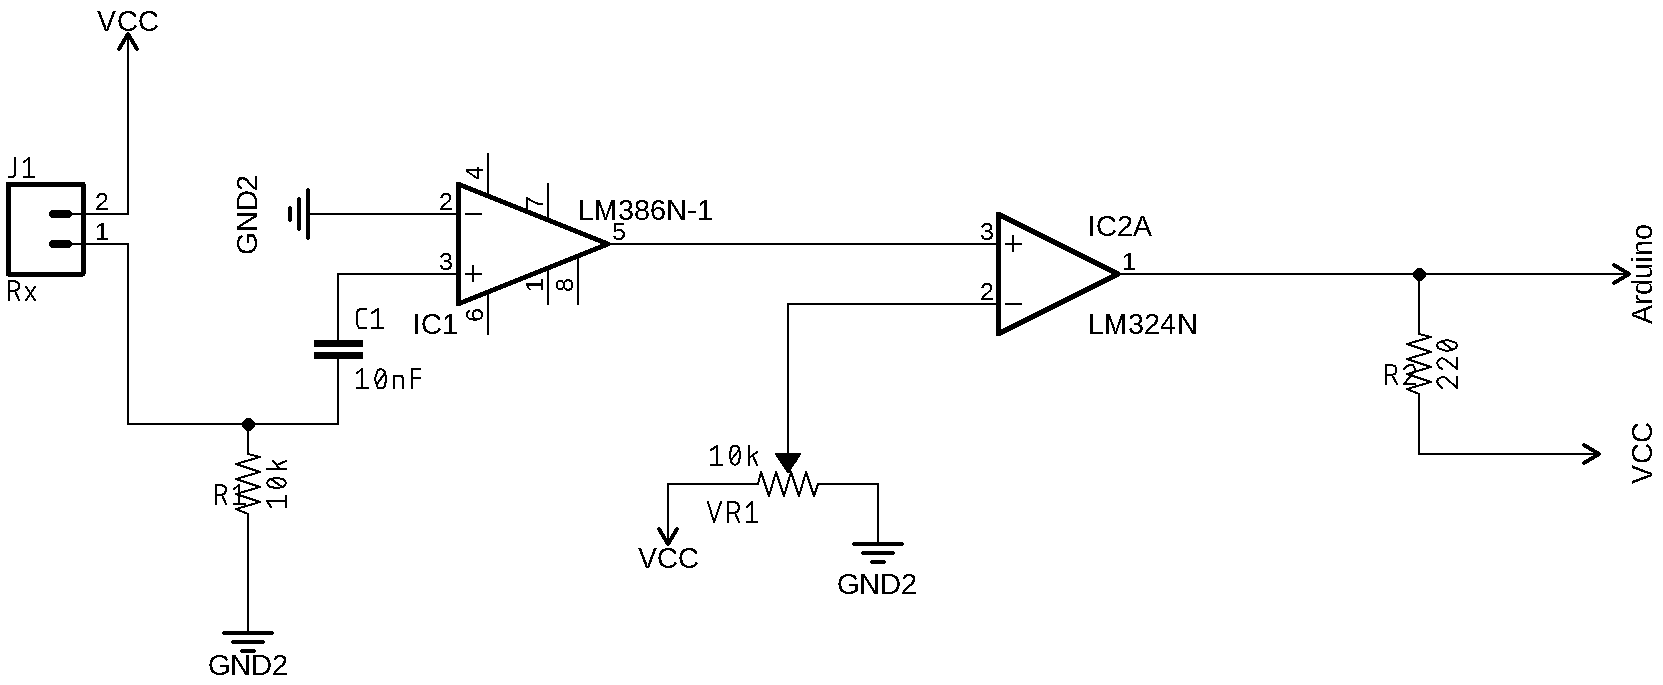
\includegraphics{rx_circuit}
\end{center}





\end{document}